\chapter{Implementation}\label{cha:implementation}
The following chapter documents the different functional modules that were implemented according to the proposal. 
The tasks related to EtherCAT compatibility and usage of RTOS are highlighted within this and the following chapter,
 as they were of higher priority.

Moreover, the functional blocks or modules interact with each other through the DSMs, which has been added as well 
as a module for its understanding.

\section{LED Control}\label{sec:leds}


In order to notify to the user the current state of each axis, the robot includes one or more LED rings. These rings are 
 a serial array of LEDs that are programmed and controlled through a serial communication protocol. Basically, the final implementation
 is an adaptation of a library that uses a PWM peripheral to generate a signal that is modulated according to the data that 
 controls the LEDs, namely digital 1s, 0s and reset as a specific duty cycle. The input pin of the first LED is connected to the MCU and depending on the modulated data, it will be 
 passed over the next LEDs, being the first LED's output the input of the next til the last component. A summary of the 
 protocol is explained in ~\cite{led_protocol}. 

Furthermore, the current LED control in the robotic system uses MCU Devices without communication capabilities leading to 
static status indication that cannot be set from the Master.

 In the next paragraphs a summary of the activities that were carried out during the implementation is presented.

\begin{description}
\item[First control tests] Learning the basics of the interface used to control one LED
\item[Code for one LED control] Using the peripherals of the MCU simple routines were written to set different basic colors in RGB. 
    The peripheral used were a two Timers (hardware libraries) to keep control of the data timing and refresh rate.
\item[Search for libraries] Once the basic communication was understood, it was clear that the usage of libraries would be more practical,
    since the first approach were not suitable for higher number of LEDs and effects; moreover, the CPU was kept busy while waiting 
    the timer state polling. The libraries found were aiming roughly either 8/16 bits processors whose main task was controlling the LEDs, 
    or more complex libraries that used DMA modules within 32-bit processor. One of the latter implemented modulation of the data over a PWM and a
    DMA peripheral for one LED strip.
\item[First library selection] Due to the inexperience working with DMA modules and as the LED control was not of a higher priority compared to other tasks, 
    it was decided to run first one of the basic libraries to achieve a multi LED control. The implementation was able to control a set of 20 LEDs
    with the processor mainly polling the Timer states.
\item[Further control tests] Despite the success of the library with one channel, the overall structure of the basic library
    was not easily portable to the proposed solution using FreeRTOS. Additionally, the DMA libraries showed afterwards being easier 
    to modify as they were designed with a more abstracted and multi-purpose approach.
\item[Second library selection] As the usage of DMA became clearer, it was decided to improve the approach by 
selecting a 32-bit processor based library, that implemented only general control functions to avoid massive code lines
related to effects and other rather unnecessary features, yet structured enough to be easily adapted. 
The final result was based upon the WS2812 Library for STM32F4 from Uwe Becker, see \cite{led_library}. 
Main modifications were the addition of multiple channels capability and global flags needed for synchronizing with DSMs.
\end{description}


\section{Temperature acquisition}\label{sec:temperature}

Similar to the LED control's library, the temperature readout needed a library to be modified to match the current project.
\begin{description}
\item[First readouts] Working with the temperature sensors was the first task in schedule, so it helped train the basic usage
    of the IDE STM32Cube, along with the hardware configuration of the MCU and the HAL libraries. 
    The sensor uses a one-wire serial protocol, which similarly to LED Control's first approach was implemented by using 
    timers for controlling 1s and 0s high levels, a continuous polling of data and a general while loop approach. 
    This method worked as intended but it was known from the beginning that it would not match the multi-tasking proposal. 
    However, it was of great importance to get to know the hardware and software, besides more functions were needed to 
    access the sensor's ROM needed e.g. for identification.
\item[FreeRTOS first tests] Short after the working code was used to do the first tests with the RTOS, 
    in this manner the code was translated as a Task (Thread as called by CMSIS) and some features like prioritization, 
    task attributes, task handling and signals were tested with other generic functions, e.g. clocks and PWM generators. 
    However, this implementation was not able to handle multiple one-wire devices due to its absence of CRC comparison.
\item[Integration of library] Finally, it was decided to adapt one open source library designed for STM32 processors. 
    This is based on the principle that UART speeds at \SIlist{9600;11200}{\bit\per\second} suit the One-Wire timing, such that the 
    detection of One-Wire devices and communication process can be downloaded to hardware already included in many 
    general-purposes processors using USART. The integration of this library is from design compatible with RTOS, 
    namely with CMSIS-RTOS. The library selected was developed by Tilen MAJERLE, review in \cite{temp_library}, and it 
    was barely modified as it contained already the desired functionalities and the development
    focused only on the integration into the DSMs and usage of it. 
\end{description}

The strategy the final library is based on is rather interesting and more details can be read in \cite{onewire_theory}.

\section{EtherCAT Slave communication: SOES adaptation}\label{sec:soes}

This functional module had the highest priority, therefore most of the effort given was focused not only 
on the library itself but the protocol and the hardware commissioning, it is hence recommendable to read through the introduction 
to the protocol in Appendix~\ref{sec:ecat_protocol}. In this sense, the current section was structure
as follows: first, a bit more technical details are presented regarding the EtherCAT specification, and some constraints for 
the prototype such that the library could be tested accordingly to the scope of the project; afterwards the EtherCAT Slave
Controller (ESC) is briefly summarized and finally, the main points of the implementation are presented.

\subsection{EtherCAT data consistency and constraints for design}\label{sec:ecat_sms}
This subsection describes both the features with which the \emph{Axis Communication Board} has compatibility, and a summary of the mechanism that the protocol
implements at the low level to work with the data exchange between Master and Slave. The constraints that were set were part of a live process that ran 
all along
the learning process of the protocol. This is important to mention, since the understanding of the protocol leads to a sinful selection of the features
that a device should have implemented. Therefore, the understanding process was a natural consequence of the integration of the SOES library. 

The reader may recall the set of Communication Profiles that are available within the EtherCAT field bus. 
A slave device must comply at least with CoE and the Mailbox, whereas the Master may comply with all the communication profiles. This of course
needs to be suited to the requirements of the application and the degree of flexibility that is to be achieved. From it, 
the Mailbox and CoE 
are the main features with which the Axis Communication Board works. Leaving aside for future integration the FoE and EoE, the former would make possible 
update the device by sending a firmware binaries to the device's bootloader; whereas the latter would make the ACB accessible for any IT tool based on TCP/IP.
Moreover, the scope of this prototype covers the Free run and SM-Synchronous mode, as they are the basic ones for communication Master-Slave, recall 
the graphical representation of synchronization modes in Fig.~\ref{fig:syncmodes}.

The Synchronization Managers play a key role, therefore the correct setup of the SMs ensure the consistency of the data and needs to be linked correctly 
depending on the specifications of each type of ESC and SW Stack that are being used, this information is also linked to the CoE Object Dictionary (OD) 
and EtherCAT Slave Information (ESI) file---a roadmap for the Slave development can be reviewed in \cite{beckhoff_slavetutorial}. 
The last mentioned activities were the main challenge within this project.


\subsection{SOES library}
%*Here comes the information about what SOES do, how is the license, what are the features that has already included, the futures that don't, how general it is, an image of its structure, the work that needs to be done*
As briefly commented in Sect.~\ref{sec:openness}, the types of licenses allow open development and integration of software. 
SOES software stack was written in C and published based upon the GPLv2, which is a Copyleft License. However, the tools developed 
by the Open EtherCAT Society which support the design, implementation and certification of EtherCAT slaves using the mentioned stack 
are commercial ones. A significant part of the challenge covered by this Project Research was to achieve the EtherCAT Slave functionality
in the prototype without those tools, as the protocols are open.
In the Table~\ref{tbl:soesrequirements} can be seen the main features abstracted and available in the stack, as well as the overall tasks to 
carry out for a device to work properly.


\begin{tuhhtable}
    \begin{tabular}[tp]{L{.3\textwidth}L{.3\textwidth}}
      \THc{1}{c}{Features} &  \THc{1}{c}{Requirements} \\
      \abovebodyrule
        EtherCAT State Machine  & Build up the SII-EEPROM Data-Layout     \\\TRc
        Mailbox Interfaces      & Create the ESI-file     \\
        CoE                     & Port libraries to the STM32 using HAL drivers     \\\TRc
        FoE + bootstrap template& Use FreeRTOS for scheduling (Hardware Requirements RAM$>$\SI{64}{\kilo\byte})     \\
      \belowbodyrule
    \end{tabular}
    \caption{Features of SOES library and the overall requirements to make it work.}
    \label{tbl:soesrequirements}
  \end{tuhhtable}


\subsection{EtherCAT Slave Controller (ESC): LAN9252} 
As part of the available hardware introduced in Chapter \ref{cha:solution}, the LAN9252-EVB-SPI is an evaluation kit for the ASIC LAN9252 manufactured by Microchip. 
This IC is an EtherCAT Slave Controller with \SI{4}{\kilo\byte} of Dual Port memory (DPRAM) and 3 Fieldbus Memory Management Units (FMMUs). 
Each FMMU performs the task of mapping logical addresses to physical addresses.
The EtherCAT slave controller also includes four SyncManagers to allow the exchange of data between the EtherCAT master and the 
local application, further technical details in ~\cite{lan9252_data}.%Reference to LAN9252 datasheet 
 As briefly summarized in Sect.~\ref{sec:ecat_sms}, each SM direction and mode of operation is configured by the EtherCAT master. Two modes of operation 
are available: buffered mode or mailbox mode. 
In the buffered mode, both the local microcontroller and EtherCAT master can write to the device concurrently. The buffer within the LAN9252 
will always contain the latest data. If newer data arrives before the old data can be read out, the old data will be dropped. In mailbox
mode, access to the buffer by the local microcontroller and the EtherCAT master is performed using handshakes, guaranteeing that no data 
will be dropped. The overall structure of the ASIC can be seen in Fig.~\ref{fig:lan92struct}. This prototype works with the buffered mode and uses SPI as Process Data Interface (PDI).

%Which mode is more efficient, what are the advantages and disadvantages?

\begin{figure}[ht]
  \centering
  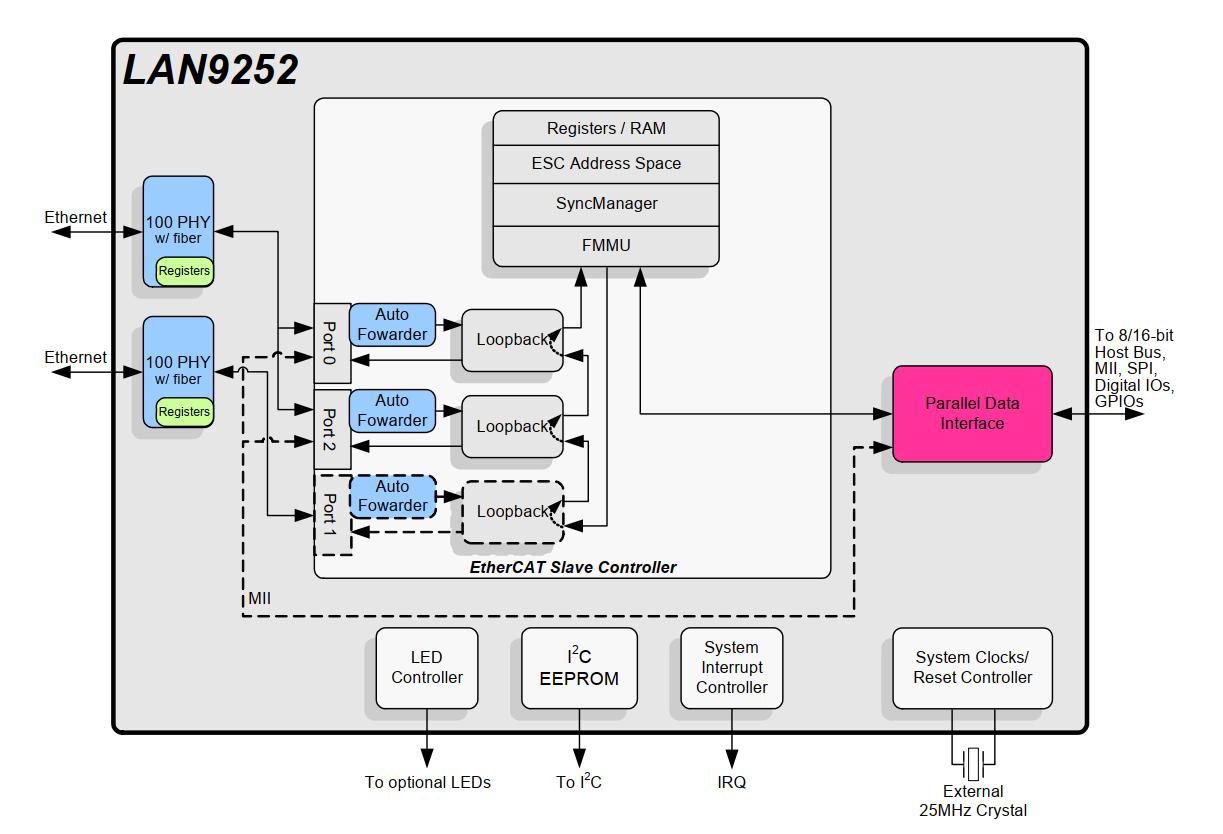
\includegraphics[width=\textwidth]{imgs/impl-lan-structure.PNG}
  \caption{Internal structure of the LAN9252, notice the PDI and EEPROM's location.}
  \label{fig:lan92struct}
\end{figure}


\subsection{Development}

Once explained the general information regarding the Communication Profile, the library and the hardware, the following lines will list and
expose some of the most relevant information during the integration. 

\begin{description}
\item[Porting of low-level functions] All the variations of functions for reading and writing ESC's registers (directly and non-directly addressed)
      are needed to be defined. HAL libraries can be used, DMA, interruption or timeout based, nevertheless, tests are required for library performance.
\item[First tests] Before integrating the SOES library, basic tests with self written functions over SPI-DMA and SPI-timeout were compared by accessing
      to test registers available in the LAN9252.
\item[Selection of the features] At the same time, in order to have the SOES library running, the features it includes needed to be selected depending on
      their usage, complexity and other things. For example, there are some MCUs that include EEPROM memory, that is mandatory for the implementation of FoE service.
      In the case of the STM32F4xx that does not have any EEPROM, the flash memory can be used instead. However, this approach represented extra effort
      in this early stage of the development. Therefore, in addition to the initial requirements, this service was avoided and the SOES integration could
      continue in a relatively lighter way.
\item[Second tests] Once understood the logic behind the library, SPI commands are sent in interruption mode and communication with the ESC was tested for the
      directly addressable registers, namely the ones related to configuration of the PHY and general chip configuration, not the ESC functions.
\item[Third tests with the Master] At this stage a compliant EtherCAT Master was configured through a PC running TwinCAT3. 
      In order to ensure a reliable configuration two different EtherCAT devices were connected synchronizing their data with the Master. Namely, 
      a commercial 3-Phase Motor Controller and an in-house multi-protocol end-effector tool. For those different devices, data structures were declared 
      and very simplistic update loops were programmed within the XAE (TwinCAT) environment using \emph{SText} programming language.
\item[Creation of an ESI file] Since the EtherCAT Core registers are indirectly addressed and only available till the ESC has been firstly readout by a 
      Master, the ESI file needs to be defined and loaded to the EEPROM of the ESC. In this way, the Master can compare and verify its compatibility and 
      the described Data Object Dictionary. The latter is closely related with the mentioned ESI file, since they are both in the same file. 
      The available information and tools provided by Beckhoff are originally designed for Beckhoff's ET1100. Microchip in turn provides some test
      examples running on PIC32 MCUs in specific development boards. The challenge was to analyze the available information to adjust the configuration
      files to the LAN9252 interfacing with the STM32 MCU. In ~\ref{app:esi_file} the main structure of the created ESI file can be consulted.
\item[Object dictionary] The object dictionary was also included in the SOES library, matching it to the one contained in the ESI file, but mapped 
    according to the few documentation available of SOES.
\item[Fourth tests] Longer tests and configuration loops were located at this stage due to the deepening on the protocol. 
Constant comparisons between the data read by the Master and the data received by the MCU host took place.
\end{description}


\section{Device State Machines (DSMs)}\label{sec:statemachines}

% Guideline
%     Introduction
%     SMS and interaction    
%     Synchronization approach, UPPAAL representation
%     Introduce the SMs what things have to be taken into account for the scheduling and prioritization

In order to have a deterministic behavior of the embedded system, a set of State Machines (DSM) -not to be confused with Synchronization Manager- 
were proposed and implemented as part of the project library. 
The DSMs software implementation follows a \emph{switch case} comparator approach, since it was simple, yet effective and flexible enough, 
to work during the prototype. 
These characteristics were very important, since the DSMs structures were in constant change as the integration of new libraries 
and the functionalities developed. 
The proposed DSMs are as follows and the diagrams can be reviewed in Appendix \ref{cha:state_machines}.

\begin{description}
\item[LED] Initializes and updates periodically the RGB value of the LED Rings. See in Fig.~\ref{fig:dsm_led}.
\item[Event Handler] Its purpose is to react to notifications or errors that could appear within other DSMs and notify to update the LED rings in accordance.
                    The approach of having defined this DSM was mainly thought for fault handling and will be the base for the inclusion of future features, e.g.,
                    receiving commands or interruption requests from any of the interfaces. See in Fig.~\ref{fig:dsm_event}.
\item[ECAT] Initializes the EtherCAT communication and activates the SOES App. It is important to mention, that this DSM is rather focused on synchronization 
            with the SOES state machine. The latter changed as the development advanced, since the native infinite loop the SOES library is based on had to be adapted.
            The two involved DSMs can be seen in Fig.~\ref{fig:dsm_ecat}.
\item[Temperature] Initializes and runs the temperature related functions. It relies primarily on the open-source library described in Sect.~\ref{sec:temperature}. 
            The DSM can be seen in Fig.~\ref{fig:dsm_temp}.

\end{description}

As to the representation of the DSM, it is important to consider the general two approaches for Finite State Machines, namely Mealy and Moore, since both 
of them provide advantages while abstracting the desire logic of the different functional blocks. In this rather practical approach the formalities are not fully
met, for instance, to choose strictly for transitions dependent on the state and inputs with actions, but using exit actions as part of each state, when it is convenient.
There are though transitions that explicitly executes a synchronization edge. This flexibility was opted due to the inherent interconnection of the DSMs
as they are not fully independent. To meet a suitable representation, the previously said is integrated with the approach of UPPAAL 
software to model timed automata and the reader is invited to look it up in \cite{uppaal_tutorial}.
As a summary, since the modelling of automata for real time systems demands a synchronization feature, this is represented and attached to the edges between 
locations---the latter in the sense that a state is a location constrained to a valuation of time and other variables---with the symbols $?$ and $!$, the former acting as 
a wait action, while the latter as a notification. Those, clearly can be understood as signals between different threads.


\subsection{Scheduling}\label{sec:scheduling_intro}

%Guidelines
% introduction
% --------------------
%     Mention the scheduling apporach of RTOS
        
%         List of proposed threads and description of them (only proposal)
%         Priority based, fixed and not based on Execution times
%            >> Time proposed for each one, mention that it is also configurable. 
%           SPI speed calculation?
%         This is a Table
     
% ---------------------This is in results-----------------------------------
%     Problems in the implementation 
%         Priority of each task + timer priority
%             Solutions + Task manager
%          Present the final table of threads
%         explains events its problems with timers, etc    
%             Solutions
%     List of resources that might demand mutex
%             List of general variables
%         Regardinf the synchronization: How the OS prevents from problems?
%             solutions
%           Future improvement (3 items for OS debugging)

In the present section, the main points regarding thread management and scheduling is presented.
All the DSMs were implemented as \emph{Threads} using CMSIS-RTOS on STM32. All threads have fixed priorities and the desired execution time
(\emph{release}) is controlled to each thread through the OS-native delay function. The previously mentioned function is not to be confused 
with the \emph{HAL} version of it, since using HW-related functions while executing an OS is conveniently avoided. The OS-function allows 
the scheduler to allocate CPU resources to any next-priority tasks. For further information regarding HAL and CMSIS implementation of delay
can be seen in ~\cite{hal_drivers} and in section \emph{Time Management} of \cite{cmsis_doc} respectively.
The time constraints are defined as \emph{desired}, since the system is
non Safety-Critical---recall the safety specification in Table~\ref{tbl:tech_specs}; hence, it has no hard real time constraint and the overall 
execution follows a best-effort approach. This, however, opens the door to further improvement in the sense of characterizing and optimizing
the reliability and task execution; the latter will be commented in Sect.~\ref{sec:scheduling_results}. 

In Table ~\ref{tbl:threads_generals} are presented the basic timing requirements depending on the functionalities of each DSM related to the thread.
Each parameter that sets up the duration can be changed in a header file, see the Appendix~\ref{appx:code}, and the individual functionality can be 
reviewed in the previous DSM section.
%**Here comes a table with the priority for each task**
\begin{tuhhtable}
    \begin{tabular}[tp]{L{.3\textwidth}C{.3\textwidth}}
      \THc{1}{c}{Thread} &  \THc{1}{c}{Release period (\si{\milli\second})} \\
      \abovebodyrule
        SOES APP SDM    & \numrange{5}{10}     \\\TRc
        LED SDM         & \num{33}    \\
        ECAT SDM*        & \num{100}     \\\TRc
        Temperature SDM & \num{1000}     \\
      \belowbodyrule
    \end{tabular}
    \caption{Basic timing requirements for threads, deadlines are rather desired since the device is non Safety-Critical. \emph{*ECAT SDM 
        is mainly event driven, nevertheless, in the connected state it has a periodic update}}
    \label{tbl:threads_generals}
  \end{tuhhtable}

A final list of priorities and threads is presented in the Table~\ref{tbl:threads_final} within Chapter~\ref{cha:results}.

%RAte monotonic oder deadline monotonic???
%EDF ----Scheduling , is this for dynamic priorities?


\section{PCB development}
%Guidelines
%   Purpose : to have a prototype
%              Altium design
%               Create a framework for hardware development
%   Based on NUCLEO 
%   Altium 3D design
%  ! Foto of real one 
%       List of issues with a simple solution
%       List of improvements
%   
%   -------------Not necessary
%   Table with, number of layers, size
%   BOM, connectors, pcb specifications
In this section straightforward information regarding the manufacturing of the PCB proposal is given.
The schematics and PCB layout can be consulted within the Appendix~\ref{appx:pcb}. The main idea around this design was introduced in Sect.~\ref{sec:pcb_proposal} 
and has the purpose of providing experience in embedded hardware design and a base work for coming projects, where
the functionalities of this prototype will be merged with other boards. Therefore, to have a physical prototype to recognize
possible opportunity areas, such as physical connectors, sizes, power source quality and signal integrity, is a corner stone for any 
future design.
The overall stages of this design are as follows:

\begin{description}
\item[Design] Altium Designer was used to prototype the PCB for this project. During the process the first approach was
                based on the open files for both the NUCLEO-F446ZE Development Board by STM and LAN9252-EVB-SPI by Microchip. By analyzing
                the general diagrams and selecting and adapting the different modules to adapt the requirements was the main challenge. To ensure
                usage of less extra devices as possible, two voltage regulators were included for \SIlist{5;3.3}{\volt}.
                To meet the routing needs a four layered PCB was selected. The final 3D model can be seen in Fig.~\ref{fig:pcb3d}.
\end{description}

\begin{figure}[ht]
    \centering
    \subfigure[ACB 3D view top]{\label{subfig:pcbtop}{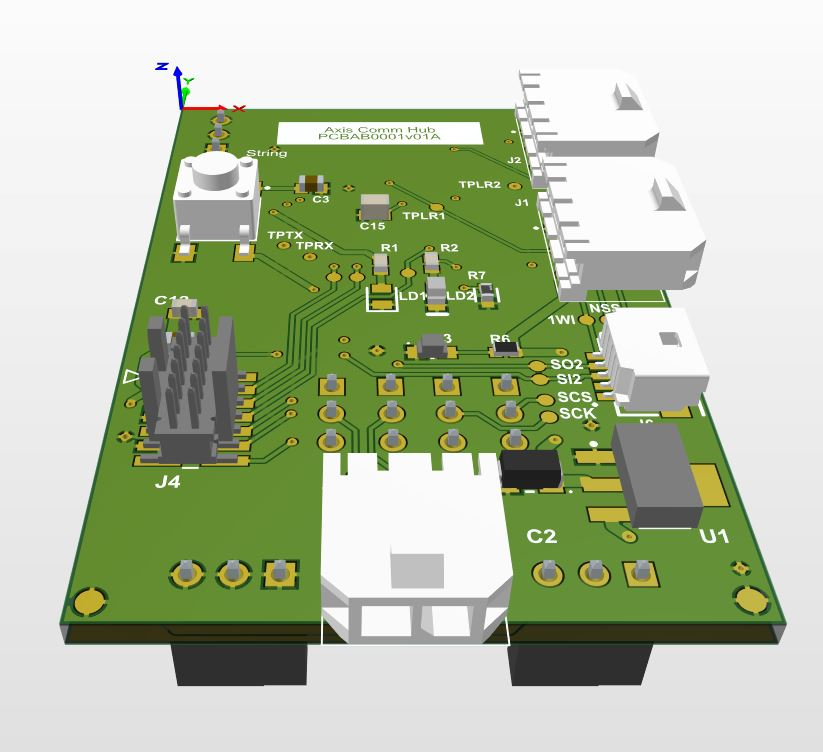
\includegraphics[width=0.4\textwidth]{imgs/pcb3d_1.JPG}}}\hfill
    \subfigure[ACB 3D view bottom]{\label{subfig:pcbbottom}{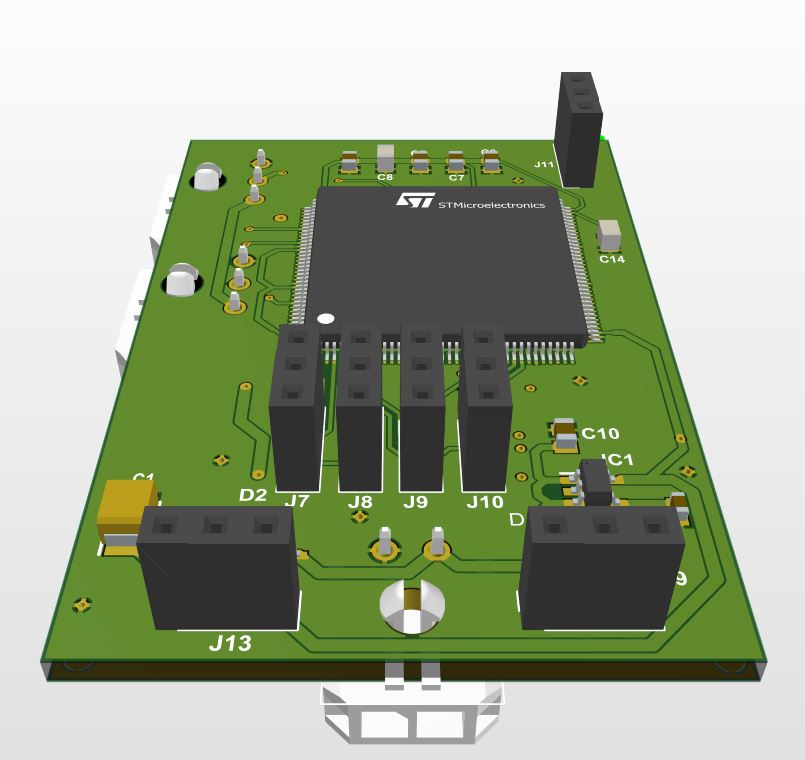
\includegraphics[width=0.4\textwidth]{imgs/pcb3d_2.JPG}}}
    \caption{3D model generated by Altium for the final design.}
    \label{fig:pcb3d}
\end{figure}


\begin{description}
\item[Manufacturing]    Due to practical reasons, the board manufacturing process was in charge of an external PCB manufacturer. In respect
                to soldering, it was made in-house.

\item[Testing I] The overall integrity and functioning of the Power-on and SWD-Programming of the STM32 MCU via SWD/JTAG connector on-board was firstly tested with good results. 
\end{description}

\begin{description}
\item[Testing II] By this stage, the readout of directly addressed memory space, specifically test and ID register, of the LAN9252 had been already done
                    with the NUCLEO board. In this manner, the code was programmed onto the ACB and so, the SPI communication gave good results. Moreover,
                    the PWM Outputs over the two channels for WS2812 LED control and the 1-wire connection were also physically tested.  
\item[Testing III] This phase is an ongoing task, since depending on the development of all the features, communication speeds and hardware 
                configurations, different scenarios are continuously emerging. A deeper analysis will be taken into account for next versions.
\end{description}



